\section{Introduction}

Software engineering has rapidly emerged as a frontier application area for large language models (LLMs).  
As models have grown more capable, they have progressed from simple program synthesis \citep{austin2021program}, to automatic code completion \citep{humaneval}, to general-purpose code generation \citep{li2022competition, lai2023ds}, to understanding code execution \citep{gu2024cruxeval}, and competition-level programming \citep{jain2024livecodebench}.  
Most recently, LLMs have demonstrated strong software engineering ability to tackle real-world issue resolution in open-source repositories \citep{swebench, sweagent, xia2025live, satoriswe}.  
To support such capabilities, more sophisticated agentic frameworks such as OpenHands \citep{openhands} scaffold LLMs with tools for search, code editing, and command execution, while agentless prompting-based approaches \citep{xia2024agentless} have shown that carefully structured prompts alone can also perform well on multi-step software engineering tasks. 

While model capabilities continue to improve, success in real-world software engineering depends not only on the underlying LLM, but also on the \emph{agent scaffold}: the orchestration, memory structures, and tool abstractions surrounding the model. Empirically, even when the same backbone model is used, different scaffolding strategies can lead to large performance disparities \citep{xia2025live}, suggesting that the design of the agent’s cognitive and operational environment is a fundamental research dimension. However, existing coding agents often rely on flat interaction histories, heuristic prompt engineering, or tightly coupled tool pipelines, which are difficult to scale to the long-horizon, multi-file, multi-step workflows characteristic of enterprise-level software engineering.
This gap is most clearly manifested in two core \textcolor{darkred}{\textbf{challenges}}:
\begin{itemize}[leftmargin=*]
    \item \textbf{\COne: Long-context reasoning.} Agents must efficiently localize relevant code within massive repositories and perform multi-hop reasoning across dispersed modules, long tool traces, and deep execution histories.
    \item \textbf{\CTwo: Long-term memory.} Agents should accumulate persistent knowledge across tasks and sessions, capturing reusable patterns, failure modes, and invariants, rather than repeatedly rediscovering information or reproducing past mistakes.
\end{itemize}
These challenges highlight that scalability in agentic software engineering requires more than longer context windows or larger models: it requires a principled approach to how agents structure, maintain, and interact with external information.



We argue that addressing these challenges requires a broader, system-level design perspective. In particular, we decompose agentic interaction into three complementary axes: \textbf{Agent Experience (AX)}, \textbf{User Experience (UX)}, and \textbf{Developer Experience (DX)}.  
AX concerns the agent’s internal cognitive workspace: how information is distilled, organized, and presented to the LLM for stable reasoning.  
UX concerns the transparency, controllability, and interpretability required for human users to understand the agent’s behavior.  
DX concerns observability, evaluation, and modularity for researchers and practitioners developing and improving agent systems.  
Most existing frameworks conflate these axes. For example, passing human-oriented logs directly into the agent’s prompt, thereby degrading AX, limiting UX, and restricting DX. Treating AX, UX, and DX as first-class and distinct design principles provides a foundation for scalable, analyzable, and reproducible agent behavior.

We first introduce the \textbf{Confucius SDK} (\Cref{fig:teaser}), an agent development platform explicitly structured around AX, UX, and DX. 
On this platform, we instantiate the \textbf{Confucius Code Agent (CCA)}, a concrete agent tailored to large-scale software engineering. 
We introduce four key mechanisms, each served for AX, UX, and/or DX, and instantiated in CCA to address the two \textcolor{darkred}{\textbf{challenges}} above:
\begin{enumerate}[leftmargin=*]
    \item \textbf{Context management (AX; \COne).}  
    A hierarchical working memory coupled with context compression enables the agent to retain essential state while supporting long-horizon reasoning without exceeding context limits.

    \item \textbf{Note-taking (AX, UX; \CTwo).}  
    A dedicated note-taking agent distills trajectories into persistent, hierarchical Markdown notes, including hindsight notes that capture failure modes, thereby supporting both durable knowledge for the agent (AX) and interpretable artifacts for humans (UX).

    \item \textbf{Extensions (AX, DX; \COne).}  
    Modular extensions define tool-use behavior, parsing, prompt shaping, and interaction policies through typed callbacks. This separation improves agent control and reasoning stability (AX) while providing observability and composability for developers (DX). CCA binds together coding-specific extensions such as file search, file editing, and CLI tools. 

    \item \textbf{Meta-agent (DX).}  
    A meta-agent automates a build-test-improve loop that synthesizes, evaluates, and refines agent configurations, enabling rapid agent development and adaptation to new environments.
\end{enumerate}

% Throughout this paper, we distinguish between the Confucius SDK and the CCA. The Confucius SDK is a general-purpose agent development platform that provides reusable abstractions for orchestration, memory, and tool use, structured around AX, UX, and DX. The CCA is a single concrete instantiation built on top of this SDK, configured specifically for large-scale software engineering tasks. Our empirical results are obtained using CCA, while the design principles and mechanisms we describe apply more broadly to agents constructed using the Confucius SDK.

To evaluate the mechanisms introduced by Confucius SDK and CCA, we conduct experiments on SWE-Bench-Verified \citep{swebench} and SWE-Bench-Pro \citep{sbp}.
CCA achieves strong performance compared with prior coding agents, demonstrating how principled scaffolding can substantially amplify the effectiveness of the same underlying LLM.
We also evaluate CCA on a custom PyTorch-Bench targeting debugging workflows on larger-scale codebases. Ablations isolate the contributions of each crucial mechanism, and analyses categorize remaining failure cases. In summary, our contributions are:
\begin{itemize}[leftmargin=*]
    \item We present the \textbf{Confucius Code Agent (CCA)}, a coding agent designed for large-scale software engineering.
    \item We present the \textbf{Confucius SDK}, a principled AX/UX/DX-balanced agent development platform with advanced context management, extensions, and long-term memory.
    \item We provide evaluations across multiple benchmarks, supported by ablations and case studies. Notably, on SWE-Bench-Pro, CCA reaches a Resolve@1 performance of \textbf{59\%}, exceeding prior research baselines and  commercial results, under identical repositories, model backend, and tool access.
    \item We empirically show that \emph{agent scaffolding}, not just model capability, is also a primary determinant of agent performance, with appropriate orchestration and memory structures outperforming stronger models.
\end{itemize}

\begin{figure*}[t]
    \centering
    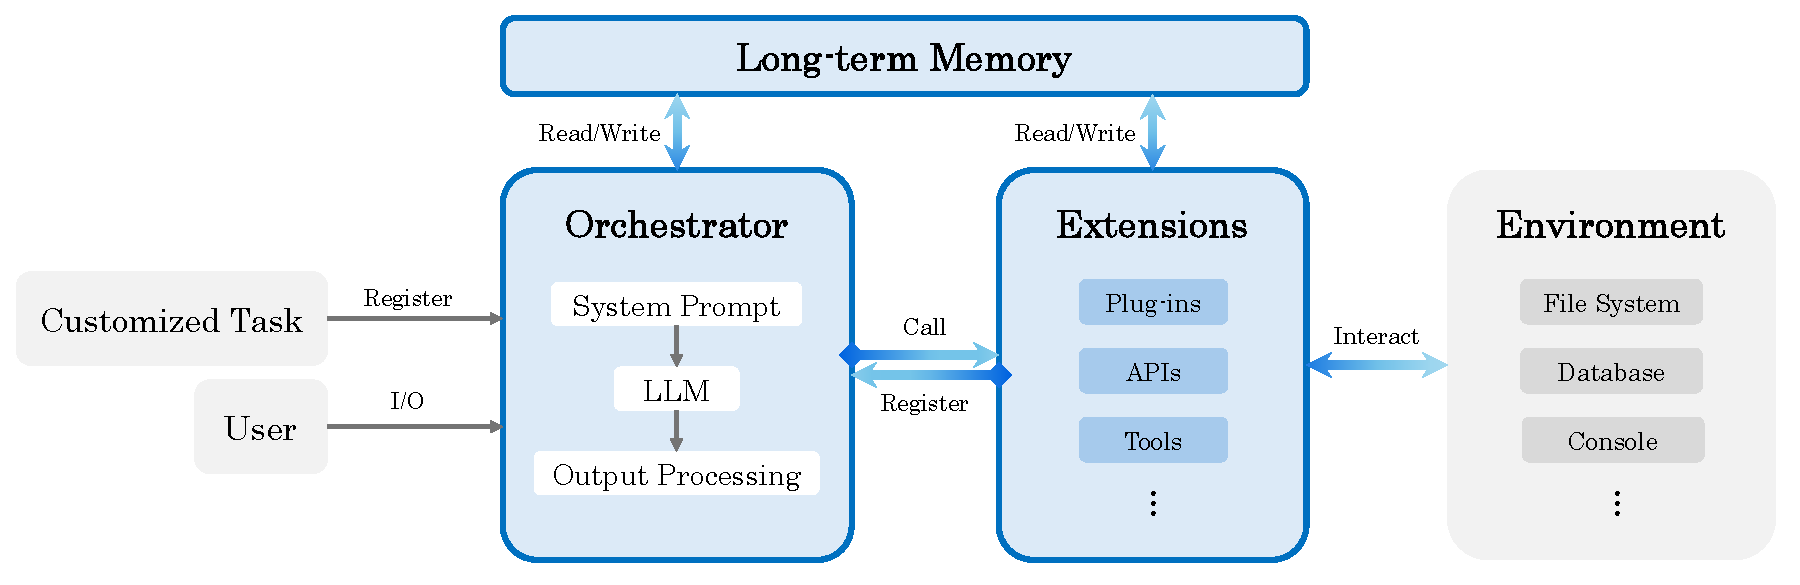
\includegraphics[width=\textwidth]{figs/teaser.pdf}
    \caption{\textbf{Confucius SDK overview.}  
    The SDK unifies an orchestrator for iterative reasoning and action execution, long-term memory for continual learning, and modular extensions for tool use and interacting with the external environment.}
    \label{fig:teaser}
\end{figure*}

